\documentclass[12pt]{article}

\usepackage[margin=1in]{geometry}
\usepackage{fancyhdr}
\pagestyle{fancy}
\usepackage{amsmath}
\usepackage{amssymb}

% limit to particular location
\usepackage{float}

% graphics
\usepackage{graphicx}
% for subfigures
\usepackage{subcaption}

% better ref links
\usepackage{hyperref}

% adjust enum layout
\usepackage{enumitem}

% footnote in footer
\newcommand{\fancyfootnotetext}[2]{%
  \fancypagestyle{dingens}{%
    \fancyfoot[LO,RE]{\parbox{7cm}{\footnotemark[#1]\footnotesize #2}}%
  }%
  \thispagestyle{dingens}%
}

\lhead{HW4}
\chead{Digital Image Processing}
\rhead{B03902036}


\begin{document}

\section*{Problem 1}
Homework required one to design an algorithm to recognize the provided grayscale CAPTCHA based on provided training set.
Three separate stages can be deduced
\begin{enumerate}[itemsep=0px]
\item Training set feature extraction.
\item CAPTCHA character isolation.
\item Character recognition.
\end{enumerate}
In the following sections, I will walk through the trial-and-error process I had gone through.

\subsection*{Trial 1}
\subsubsection*{Training set feature extraction}
We are interested in the characters themselves, a mask with ones on the characters is closer to expectation. Trivial observation indicates no significant noise exists, and gray level is marginal to non-existence along character edges, we can try to threshold it directly by averaging global minimum and maximum. 
\begin{equation}
T = \sum_i \sum_j \frac{max(I(i, j))-min(I(i,j))}{2}
\end{equation}
Due to the fact that {\tt TrainingSet.raw} is provided as black-on-white style, thresholding criteria is reversed.
\begin{equation}
I(i, j) = 
\begin{cases}
	1, I(i, j) < T \\
	0, I(i, j) \geq T
\end{cases}
\end{equation}

\begin{figure}[H]
    \centering
    \begin{subfigure}[t]{0.5\textwidth}
        \centering
        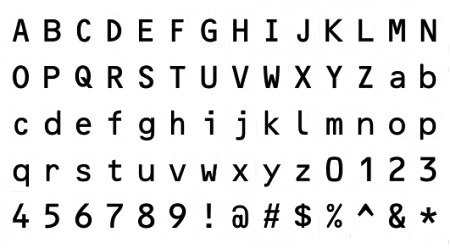
\includegraphics[height=1.5in]{images/training_original}
        \caption{Grayscale}
    \end{subfigure}%
    ~
    \begin{subfigure}[t]{0.5\textwidth}
        \centering
        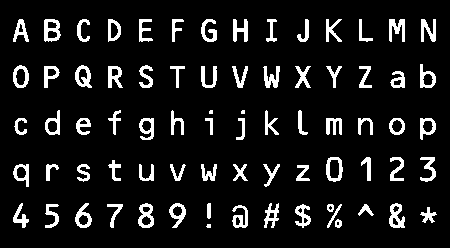
\includegraphics[height=1.5in]{images/training_binary}
        \caption{Binary}
    \end{subfigure}
    \caption{Pre-processed training set}
\end{figure}

The training set characters are displayed in montage, we need to isolate them to individual characters before proceeding to next step. The montage contains 14-by-5 characters, with consistence spacing between horizontal and vertical neighbors. We can easily calculate the appropriate spacing to separate them.
Margins of the image can causes misalignment after cropping, margin size of 5 and 7 pixels are empirically chose for horizontal and vertical edges respectively.

\begin{figure}[H]
    \centering
    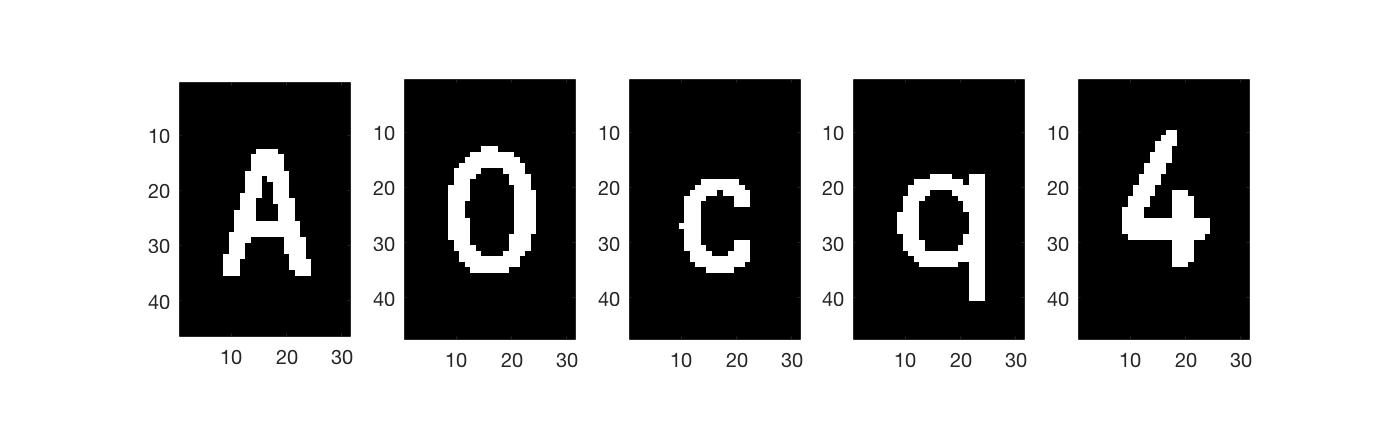
\includegraphics[width=0.7\textwidth]{images/training_cropped_col1}
    \caption{Cropped characters, first column is shown.}
\end{figure}

To perform further processing, I choose to resize them to image of size 32-by-32 pixels to ease the process.

\begin{figure}[H]
    \centering
    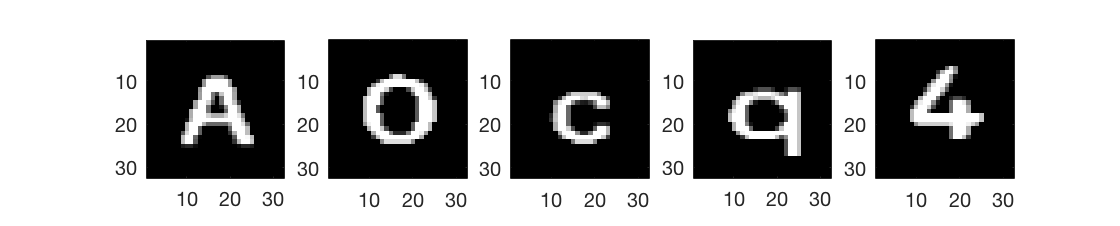
\includegraphics[width=0.7\textwidth]{images/training_resized_col1}
    \caption{Resized characters to square, first column is shown.}
\end{figure}

Characters seem to have enough differences from scanline perspective, therefore, I project sum each character along horizontal and vertical direction to derive their 2-by-32 feature vector in \autoref{fig:feature_direct_mip}.

\begin{figure}[H]
    \centering
    \begin{subfigure}[t]{0.5\textwidth}
        \centering
        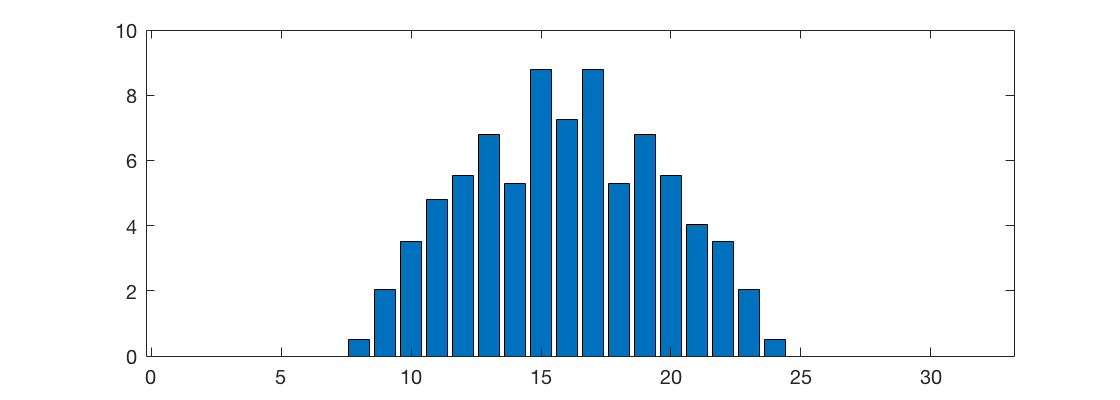
\includegraphics[height=1in]{images/feature_x_mip_a}
        \caption{X direction}
    \end{subfigure}%
    ~
    \begin{subfigure}[t]{0.5\textwidth}
        \centering
        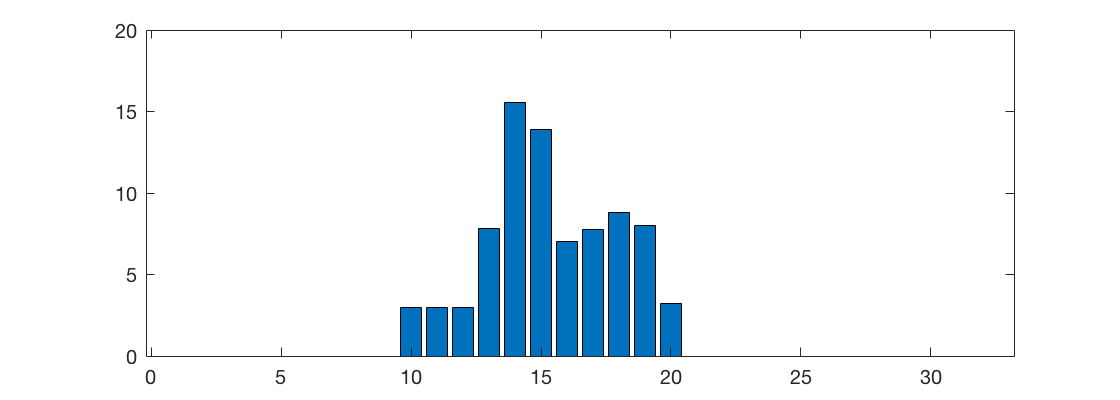
\includegraphics[height=1in]{images/feature_y_mip_a}
        \caption{Y direction}
    \end{subfigure}
    \caption{Cumulative sum projection of A}
    \label{fig:feature_direct_mip}
\end{figure}

\subsubsection*{CAPTCHA Character isolation}
Both sample images are easy to process as the training set. 

\begin{figure}[H]
    \centering
    \begin{subfigure}[t]{0.5\textwidth}
        \centering
        
\includegraphics[height=1in]{images/sample1_binary}
        \caption{Sample 1}
    \end{subfigure}%
    ~
    \begin{subfigure}[t]{0.5\textwidth}
        \centering
        
\includegraphics[height=1in]{images/sample2_binary}
        \caption{Sample 2}
        \label{fig:sample2_no_threshold}
    \end{subfigure}
    \caption{Binary sample images}
\end{figure}

Sadly, {\tt sample2.raw} contains unwanted speckle noises, visualized in \autoref{fig:sample2_no_threshold}. Therefore, median filter is applied specially for it. Kernel size of 3 is arbitrarily chosen by trials.

\begin{figure}[H]
    \centering
    \begin{subfigure}[t]{0.5\textwidth}
        \centering
        
\includegraphics[height=1in]{images/sample2_binary}
        \caption{Before}
    \end{subfigure}%
    ~
    \begin{subfigure}[t]{0.5\textwidth}
        \centering
        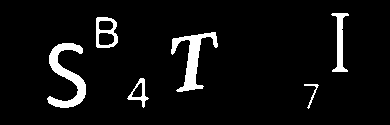
\includegraphics[height=1in]{images/sample2_binary_filtered}
        \caption{After}
    \end{subfigure}
    \caption{Median filter for {\tt sample2.raw}}
\end{figure}

For efficient labeling of connected components, disjoint-set algorithm based on handouts of Duke University {\it CS100e: Program Design and Analysis II} (\url{https://www2.cs.duke.edu/courses/cps100e/fall09/notes/UnionFind.pdf}) is used. However, characters such as {\tt i} will be labeled as separate components, hence, dilation is first performed prior to the labeling, and masked out dilated regions later on. Dilation kernel size is empirically chosen to be 7. 8-connected component is used.

\begin{figure}[H]
    \centering
    \begin{subfigure}[t]{0.5\textwidth}
        \centering
        
\includegraphics[height=1in]{images/sample1_labeled_dilated}
        \caption{Regions dilated}
    \end{subfigure}%
    ~
    \begin{subfigure}[t]{0.5\textwidth}
        \centering
        
\includegraphics[height=1in]{images/sample1_labeled_masked}
        \caption{Masked result}
    \end{subfigure}
    \caption{Character labeling ({\tt sample1.raw})}
\end{figure}

Using labels, we can crop out each characters and sort them according to their horizontal position, implicit requirement for English reading convention.

\begin{figure}[H]
    \centering
    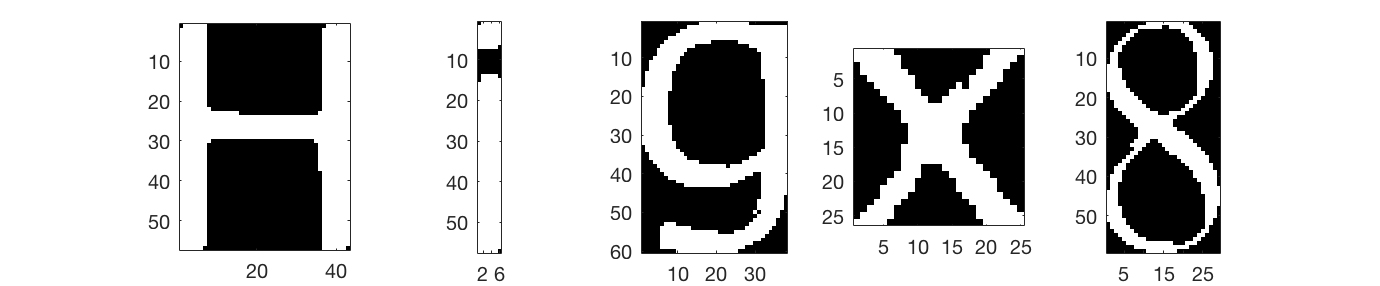
\includegraphics[width=0.7\textwidth]{images/sample1_cropped}
    \caption{Cropped characters}
\end{figure}

At last, characters are resized to 32-by-32 squares as well, same goes for {\tt sample2.raw}.

\begin{figure}[H]
    \centering
    \begin{subfigure}[t]{0.5\textwidth}
        \centering
        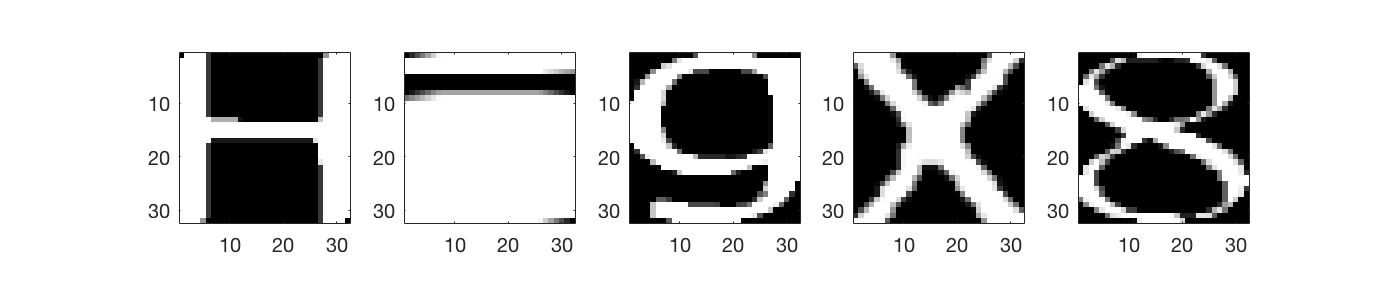
\includegraphics[width=\textwidth]{images/sample1_resized}
        \caption{{\tt sample1.raw}}
    \end{subfigure}%
    ~
    \begin{subfigure}[t]{0.5\textwidth}
        \centering
        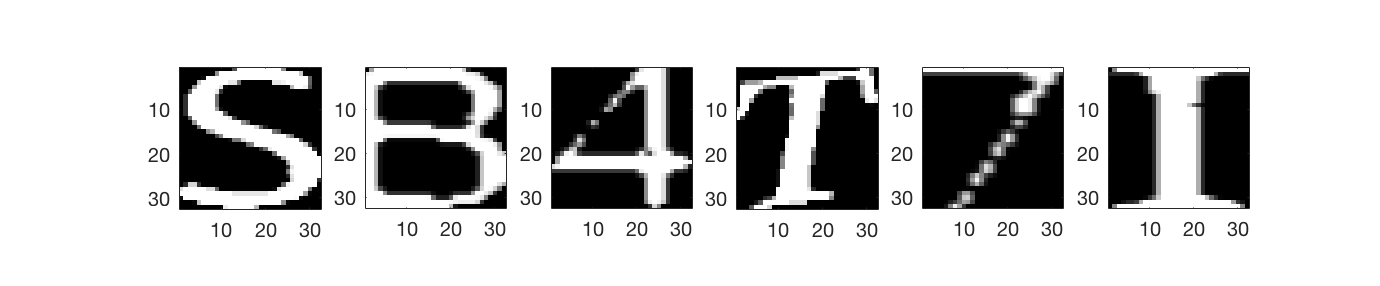
\includegraphics[width=\textwidth]{images/sample2_resized}
        \caption{{\tt sample2.raw}}
    \end{subfigure}
    \caption{Resized characters}
\end{figure}

\subsubsection*{Character recognition}
Directly subtract the differences between projection sum, I can retrieve the difference between curves, and use it as an index to find out which character is the most similar.

\begin{equation}
\begin{cases}
	d_x = \sum \vert \vec{c_x} - \vec{t_x} \vert^2 \\
	d_y = \sum \vert \vec{c_y} - \vec{t_y} \vert^2 \\
\end{cases}	
\end{equation}
where $\vec{c}$ is the feature character of CAPTCHA characters, while $\vec{t}$ is the feature character of training template. $d_x$ and $d_y$ are scalars. All the vectors are normalized prior to operations. A unified distance metric is used 
 \begin{equation}
 	d = \sqrt{d_x^2 + d_y^2}
 \end{equation}
 
\subsubsection*{Evaluation}
100\% error on both image.

\subsection*{Trial 2}
\subsubsection*{Training set feature extraction}
After reviewing the source code, I realize training set did not stretch the characters. Therefore 
\begin{figure}[H]
    \centering
    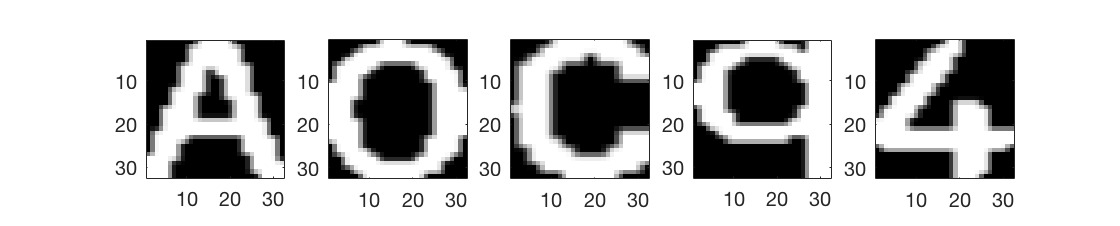
\includegraphics[width=0.7\textwidth]{images/training_resized2_col1}
    \caption{Stretched}
\end{figure}

\subsubsection*{Evaluation}
90\% average error rate. Only {\tt H} is correctly recognized in {\tt sample1.raw}. Apparently, direct curve comparison is not feasible. 

\subsection*{Trial 3}
\subsubsection*{Character recognition}
If we accumulate the projection result again, then the normalization to acquire the distance metric is essentially calculating the cumulative distribution function for pixel intensity along different direction (horizontal and vertical). By treating the problem as a binary classifier system, we can utilize the receiver operating characteristic (ROC) curve, but instead of favoring true positive direction, which requires maximizing the ROC curve area over $y=x$ line, we try to {\it minimize} that area, since same character should not deviate its distribution along any axis.

Feature vectors along both axis are now treated as sample points along X and Y direction, which are linearly interpolated to uniform X grid of size 32. The rationale of 32 is due to the resampled image size, applied earlier, is 32-by-32.

We can formulate the calculation of ROC area as 
\begin{equation}
	A_{ROC} = \sum \vert \vec{c} - \vec{t} \vert
\end{equation}

\subsubsection*{Evaluation}
{\tt sample1.raw} now has 60\% error rate ({\tt H\^{}gSD}). {\tt sample2.raw} now has 83\% error rate ({\tt 2O9tYI}). Average error rate 72\%. If we can loosen the restriction and treat upper and lower cases as the same, then average error rate drop to 64\%.

\subsection*{Trial 4}
\subsubsection*{Character recognition}
After reading Wikipedia about template matching, I decided to drop the sum projection shit and use sum of absolute differences ($SAD$). 
\begin{equation}
	SAD(i, j) = \sum_i \sum_j \vert I(i, j) - T(i, j) \vert
\end{equation}
where $I$ is the sampled CAPTCHA character, while $T$ is the training set template. No more fancy processing, not even correlation

\subsubsection*{Evaluation}
{\tt sample1.raw} now has 20\% error rate ({\tt H\&gXS}). {\tt sample2.raw} now has 0\% error rate ({\tt SB4T7I}). Average error rate 10\%. 

\end{document}
              